\documentclass{standalone}
\begin{document}
	\subsection{Gold Standard}
	
	In order to obtain quantitative measures about the performances of the developed pipeline, I have compared the results with the manual annotation provided by the Department of Diagnostic and Preventive Medicine of the Poloclinico Sant'Orsola - Malpighi. 
	
	The comparison was made using sensitivity and and specificity scores. 
	\paragraph{Sensitivity} refers to the ability to correctly detect ill areas. It is defined as the number of voxel classified as lesions among all the lesions. in other world is defined as the number of true positives over the total number of lesions voxels (True POsitives + False negtives) : 
	\begin{equation}\label{eq:sensitivity}
		Sensitivity : \frac{True Positive}{True Positive + False Negatives}
	\end{equation}

	\paragraph{specificity} relates to the  ability to correctly reject healthy areas. Is defined as the number of rejected pixels(True Negative) agains the total numner of healthy areas (True Negative + False Positives) : 
	\begin{equation}
		spcificity : \frac{True Negative}{True Negative + False Positives}
	\end{equation}
	
	As ground truth I have considered the $5$ gold standard segmentations.
	
	The results of these measures are displayed in table\,\ref{tab:Measures}
	\begin{table}[h!]
		\centering
		\begin{tabular}{|c|c|c|c|c|}
			\hline
			\multirow{2}{*}{}		  & \multicolumn{2}{c|}{Predicted} & \multicolumn{2}{c|}{Annotation} \\ \hline
						& Sensitivity & Specificity	 		& Sensitivity & Specificity		 \\ \hline
			Patient 1	& $0.412$	  &	$\sim 1.00$			&	$0.676$	  &	$ 0.999$ 		 \\ 
			Patient 2	& $0.399$	  & $\sim 1.00$ 		&	$0.698$	  & $ 0.995$		 \\
			Patient 3	& $0.570$	  &	$\sim 1.00$			&	$0.653$	  & $ 0.999$		 \\
			Patient 4	& $0.512$	  & $\sim 1.00$			&	$0.325$	  & $ 0.999$		 \\
			Patient 5 	& $0.628$	  & $\sim 1.00$			&	$0.974$	  &	$ 0.999$		 \\ \hline
		\end{tabular}\caption{Sensitivity and Specificity for the pipeline segmentation and annotation. As a ground truth was used a sem-automatic segmentation made and evaluated by $5$ experts with at least $2$ years of experience.}\label{tab:Measures}
		
	\end{table}
	
	
	The first thing we can notice is that the segmentation performances achieved by the semi-automatic method seems to have better quality perfomances, achieving a better capability to detect lesion areas. However we have to point out that the semi-automatic method requires several hours and the involved of trained experts. The proposed pipeline requires only few minutes and no trained personnel.
	
	We have also to point out that the achieved semiautomatic segmentation is subject on the experience of the operator. Only few patients per days may be segmented without lack of performances, since after several subsequent segmentation the level of concentration will drop.
	
	
	 
	We have also to point out that the developed pipeline may segment several patient without lack of performances. The training personnel may segment only one or two patient per days, 
	
	The specificity values allow us to think that the developed pipeline doesn't produce an high number of false positives. The  sensitivity may suggest that some lesion areas may be missed. We will see that each area is identified, however there is an uderestimation of the total lesion volume. 
	

 		\begin{figure}[h!]
 		\centering
 				\subfigure[Ground truth for Axial, sagittal and coronal view of the first patient]
 				{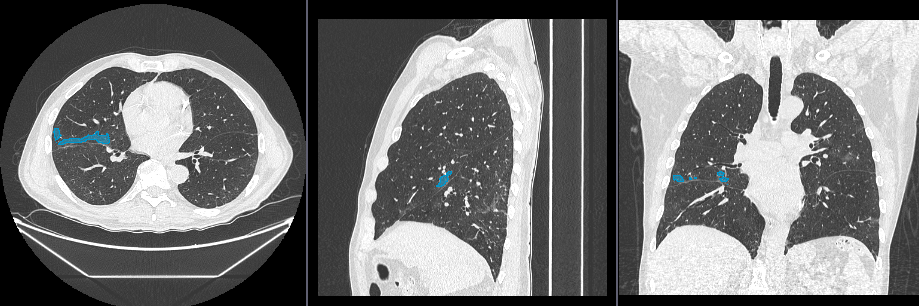
\includegraphics[scale=.4]{PATIENT1_GT.png}}
 		%\hspace{1mm}
 				\subfigure[Predicted lesions areas for Axial, sagittal and coronal view of the first patient]
 				{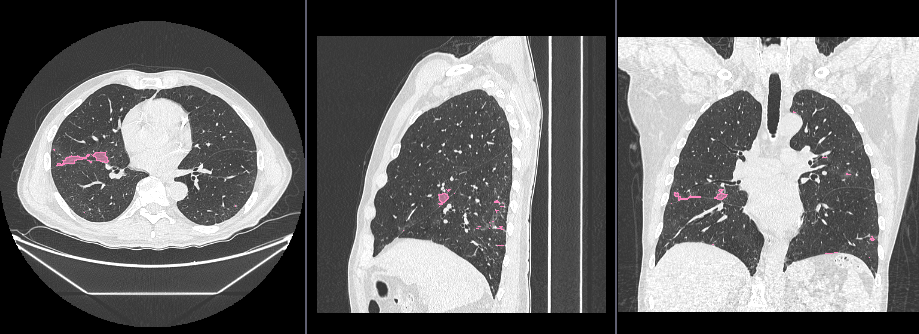
\includegraphics[scale=.4]{PATIENT1_PR.png}}
 			\caption{Comparison between the gold standard segmentation(blue) and the pipeline results(pink) for axial, sagittal and coronal view of a patient with a low involvement of lung parenchima. We can see that te main lesion areas are identified, even if an understimation of the total volume is present together with some small misclassified points.}\label{fig:pat1}
 		\end{figure}
 	
 	In \figurename\,\ref{fig:pat1} I've reported a comparison between the ground truth (blue) and the pipeline segmentation (pink) for the first patient in axial, sagittal and coronal view. We can see how the main lesion areas are correctly identified, however a low underestimation of the total lesion volume is presents, toghether with the presence of false positives in the lowest back regions. This is a particular case, since the involvement of lung volume is very low, as well as the contrast between lesions and healthy lung.
 	
 	
 		\begin{figure}[h!]
 			\centering
 				\subfigure[Ground truth for Axial, sagittal and coronal view of the third patient]
 						{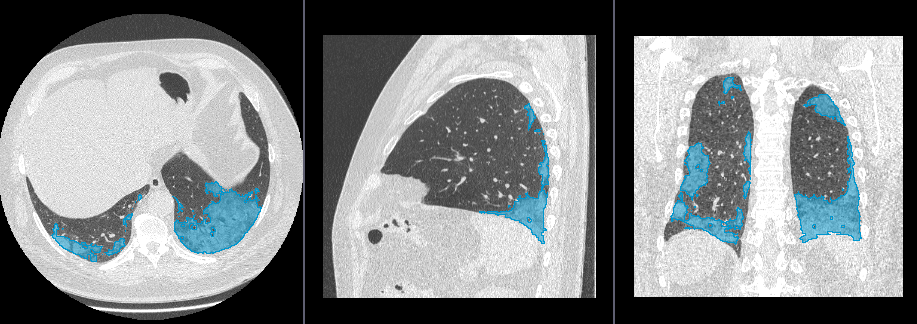
\includegraphics[scale=.4]{PATIENT3_GT.png}}
 		%\hspace{1mm}
 				\subfigure[Predicted lesions areas for Axial, sagittal and coronal view of the third patient]
 						{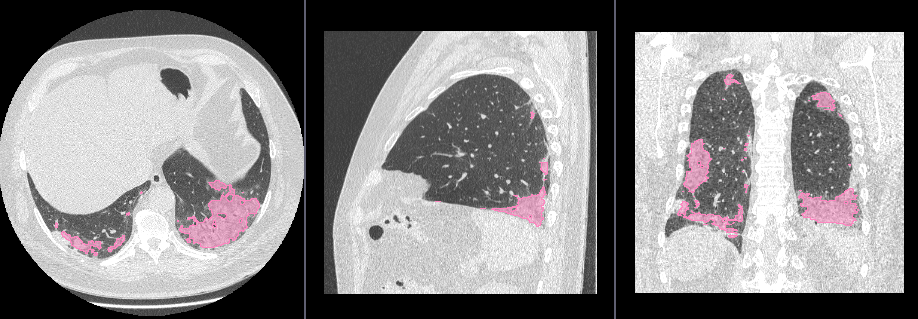
\includegraphics[scale=.4]{PATIENT3_PR.png}}
 		\caption{Comparison between the gold standard segmentation(blue) and the pipeline results(pink) for axial, sagittal and coronal view for a patient with a large involvement of lung parenchima. We can see how the lesion areas are correctly identified}\label{fig:pat3}
 		\end{figure}
 	
 	In \figurename\,\ref{fig:pat3} I've reported a comparison between the ground truth (blue) and the pipeline segmentation (pink) for the third patient in axial, sagittal and coronal view. The patient presents an high involvement of lung regions.  The lesion areas, which  in this case presents an high contrast with the lung regions, are correctly selected. In this case no misclassified points are detected. This suggest that the pipeline is able to correctly identify the lesion areas. 
 	
 	
	
\end{document}